\chapter{Flow alignment}
\label{cha:45}
\section{Introduction}
It is fair to say that the number of predictions, implications and questions that arise from the analysis of any dynamic theory of liquid crystals seems to be almost endless. This, along with the sheer amount of experiments that one could dream up to test these predictions, makes the study of liquid crystal dynamics a vast and interesting area of research. As such, in this chapter introductory experimental work carried out on the pressure driven flow alignment of a nematic liquid crystal exhibiting planar homogeneous alignment is presented.

In this study the director reorientation under pressure driven flow has been observed primarily for an initial alignment condition of $\phi_0=45^{\circ}$ (the director is aligned at $45^{\circ}$ to the direction of flow through a rubbed polymer layer). The reorientation of the director by the flow field is observed by means of optical conoscopy, and a comparison is made between the rotation of the experimental figures and the rotation of simulated figures. Simulated figures are constructed from director profiles calculated using the dynamic theory of Ericksen, Leslie and Parodi as described in Section \ref{sec:theory}. An analysis of the $\theta$ and $\phi$ director profiles as a function of position in $z$ and flow rate will also be presented. A good level of agreement between the one dimensional model and the experimental results is shown.

\section{Azimuthal alignment}
When conducting any experiment that examines the behaviour of a nematic liquid crystal (and liquid crystals in general), there is a vast range of initial director profiles that can be chosen for a cell, with each one creating a distinct alignment state of the director for the measurement of a particular property of that liquid crystal. For example, much work has been carried out in the Exeter group on the dynamics of Hybrid Aligned Nematic (HAN) cells \cite{Jewell2003,Jewell2004,Jewell2005,Yang2007,Jewell2002a}. For HAN cells, the director is given planar alignment on one surface (conventionally by a buffed polymer layer) and vertical alignment (conventially from lecithin dissolved in ether) on the other. In HAN cells, the strength of the bend and splay distortions result in a threshold-less response to applied electric fields. This means that very small voltages will substantially distort the highly sensitive director\footnote{The HAN cell is also of commercial interest as it is one of the stable states of the Zenithal Bistable Device.}.

When considering experiments involving the flow of a nematic liquid crystal, the three principal orientations of the director that one may consider, are those of the Miesowicz viscosities (shown schematically in Figure \ref{fig:eta}). Much like in the HAN cell, a liquid crystal flow cell can also be designed to have different combinations of alignment on the inner surfaces, with these different alignments allowing for examination of different flow properties of the liquid crystal. 

The primary focus of this chapter is the case of a flow cell exhibiting planar homogeneous alignment at an azimuthal angle of $\phi_0=45^{\circ}$ to the direction of flow. That is, a cell where the director is initially aligned to be planar through the cell $\left(\theta=90^{\circ}\right)$ at an angle of $45^{\circ}$ to the flow direction on both the lower and upper cell walls. Following from the theoretical analysis in Chapter \ref{sec:theory}, we know that the steady state alignment angles for flow-aligning nematic liquid crystals are those of $\phi=0^{\circ}$ and $\theta=\theta_l$. That is, alignment with the long axis of the liquid crystal molecules parallel to the flow direction and tilted up by a small angle out of the $x-y$ plane. Therefore, a pertinent question is to ask, \textit{how do we expect the director to achieve these steady state alignment angles if it is originally aligned in a different geometry?}

In order to answer this question, one may look at the work of Van Horn \textit{et al} \cite{Boudreau1999,Horn2003,VanHorn2000}. Here, common nematic liquid crystals such as 4-cyano-4'-n-pentylbiphenyl (5CB) and N-(4-methoxybenzylidene)-4-butylaniline (MBBA) have been made to flow by means of a shearing motion (with the liquid crystal sandwiched between two glass plates, where one plate is sheared relative to the other). For both of these flow aligning nematic liquid crystals, the director has been observed to distort away from the initial planar homogeneous alignment condition of both $\phi_0=90^{\circ}$ and $\phi_0=45^{\circ}$, towards the steady state azimuthal angle of $\phi=0^{\circ}$. In the case where the director is initially aligned at $\phi_0=0^{\circ}$ (parallel to the flow direction), there is no observed rotation of the director, as it is already in the steady state condition \cite{Boudreau1999}. Similarly, in terms of $\theta$, the director is seen to come to the steady state Leslie angle of approximately 9$^{\circ}$ out of the $x-y$ plane for 5CB and 8$^{\circ}$ out of the $x-y$ plane for MBBA. This is seen to happen through the depth of the cell. Importantly, the rate and manner in which the director distorts to achieve the steady state azimuthal alignment angle of $\phi=0^{\circ}$ is also shown to depend on the value of the initial alignment angle $\phi_0$. This has been observed before, and will be discussed a little later in Section \ref{pg_instability}. The manner in which the director is suggested to distort under pressure driven flow is the focus of the analysis in this chapter, and will also be discussed in the following section in terms of simulation from the one dimensional model.

\subsection{Simulated pressure driven flow}
\label{sec:simulated_flow}
For the case of pressure driven flow, Figure \ref{fig:different_phis} shows the computed \textit{mean} azimuthal rotation of the director for the liquid crystal 5CB calculated by the dynamic one dimensional model described in Chapter \ref{sec:theory}. In this figure, the mean value of the azimuthal rotation is plotted as a function of the volumetric flow rate for a flow cell that is 50 $\mu$m thick with both surfaces initially aligned at the azimuthal angle $\left(\phi_0\right)$ indicated by the 0 $\mu$L/h flow rate in Figure \ref{fig:different_phis}. As was discussed in Chapter \ref{sec:theory}, given a series of pressure gradients, the one dimensional model computes a series of tilt, twist and velocity profiles. The volumetric flow rates from simulation are calculated in turn from these velocity profiles. This figure has been included to give a feel for the general trend in the average director rotation for a flow aligning nematic liquid crystal, as has been predicted by the theory of Ericksen and Leslie and Parodi.

To begin with, it is worth noting that Figure \ref{fig:different_phis} shows very similar trends to those experimentally measured by Van Horn \textit{et al}, albeit for a shear flow regime. In Figure \ref{fig:different_phis} we see the expected behaviour that all curves (regardless of the initial azimuthal alignment) tend towards the steady state azimuthal angle of $\phi=0^{\circ}$ as the flow rate is increased (or the rate of strain on the director in reference \cite{Boudreau1999}).\footnote{Note that here we are plotting the average azimuthal distortion,  and as such, the curve will never fully reach $\phi=0^{\circ}$ due to the thin layers at the surfaces of the cell retaining their initial alignment angle. However, at very high flow rates, the vast majority of the cell has rotated towards $\phi=0^{\circ}$.}

For flow in a cell that has an initial alignment of $\phi_0=0^{\circ}$, parallel to the flow direction (the black line), it is seen that there is no average rotation of the director. This, as described above, is due to the fact that the director initially starts in the steady state alignment angle of $\phi=0^{\circ}$. This result has been experimentally measured in reference \cite{Boudreau1999} and also in this study. In this case, as there is no rotation in $\phi$, the director will only undergo a $\theta$ rotation. The details of which will be discussed in Section \ref{sec:tilt_alignment}.

\begin{figure}
\begin{center}
\includegraphics[width=0.7\textwidth]{Figures/45/vary_phi}
\end{center}
\caption[Average director rotation for varying values of $\phi_0$]{\label{fig:different_phis} Computed mean azimuthal rotation of the director as a function of the volumetric flow rate for varying values of $\phi_0$. Curves are calculated for a 50 $\mu$m thick, homogeneously aligned liquid crystal cell $\left(\theta_0=90^{\circ}\right)$ with initial azimuthal alignment $\left(\phi_0\right)$ ranging from 0 to 80$^{\circ}$. The difference in distortion profile from $\phi_0=0^{\circ}$ to $\phi_0=89^{\circ}$ is clear.}
\end{figure}

As the initial azimuthal alignment angle is increased, it is seen in Figure \ref{fig:different_phis} that the average azimuthal motion of the director tends to pull away from the initial alignment angle and rotate towards the steady state angle of $\phi=0^{\circ}$ as the flow rate is increased. This rotation is not seen to occur in a linear fashion, where the shape of the transient portion of the curve changes as a function of the initial alignment angle. This response, as will be discussed later, is due to the competing interaction between the viscous torque from flow and the elastic restoring torque created by the surface alignment layer at the cell boundaries.

\subsection{The Pieranski-Guyon instability}
\label{pg_instability}
Perhaps most interestingly, as is discussed above, a distinct change in the shape of the curve is seen as the initial azimuthal alignment angle is changed towards values approaching normal to the flow direction ($\phi_0=90^{\circ}$).

This is best demonstrated in Figure \ref{fig:Pieranski_Guyon_instability}, which shows a magnified version of Figure \ref{fig:different_phis}, with initial alignment angles ranging from $\phi_0=89^{\circ}$ to $\phi_0=89.999^{\circ}$. In this figure it is shown that for an initial alignment of $\phi_0=89^{\circ}$, the director rotates, on average, very little at the lowest flow rates, eventually distorting towards the steady state alignment angle of $\phi=0^{\circ}$. As the initial azimuthal alignment angle is increased to values of $\phi_0=89.99^{\circ}$ and $\phi_0=89.999^{\circ}$, this non-linear response is further exaggerated, with a critical flow rate being required before any azimuthal rotation is observed at all (in this case, this is shown by a sharp threshold behaviour in the $\phi_0=89.999^{\circ}$ line at a volumetric flow rate of approximately 12 $\mu L/h$). This extraordinary effect, which has been described as a `\textit{hydrodynamic analogue of the Freedericks transition}' was first experimentally observed by Pawel Pieranski and Etienne Guyon in 1973 \cite{Pieranski1973} and is often referred to as the Pieranski-Guyon instability.

In their experiment, a sample of the nematic liquid crystal MBBA aligned at $\phi_0\approx90^{\circ}$ (normal to the flow direction) was sheared between two glass plates whilst being probed by a conoscopic beam (historically, most flow experiments in this field had been conducted by shearing one of the bounding plates relative (and parallel) to the other, creating a linear velocity distribution across the depth of the cell \citep{Boudreau1999,Horn2003,VanHorn2000,Graf1992,Borzsonyi1998,Kemp1971}). In their experiment, they observed a critical rate of shear, below which no rotation of the conoscopic figure was observed. This result was explained by the symmetry of the geometry, whereby, with the director aligned planar homogeneously and normal to the flow direction, there is no hydrodynamic torque on the nematic molecules, resulting in no distortion at low rates of shear \cite{Pieranski1973}. As the shear rate is increased much further, the conoscopic figure is observed to rotate (associated with azimuthal rotation of the director) and also translate (associated with tilting of the director). These distortions were seen to be stable at any given continuous shear rate.

\begin{figure}
\begin{center}
\includegraphics[width=0.7\textwidth]{Figures/45/pieranski}
\end{center}
\caption[The Pieranski-Guyon instability]{\label{fig:Pieranski_Guyon_instability} The Pieranski-Guyon instability. Computed distortions are shown (as in Figure \ref{fig:different_phis}) for varying values of $\phi_0$ close to 90$^{\circ}$. As $\phi_0$ approaches 90$^{\circ}$, the Pieranski-Guyon instability is seen, whereby there is no azimuthal rotation of the director at low flow rates. This instability is explained by the stable solutions to the dynamic equations of $\phi=90^{\circ},\theta=90^{\circ}$.}
\end{figure}

As explained by Pieranski, in order for the instability to exist, there needs to be a small fluctuation of the director away from the planar homogeneous alignment condition. This small displacement then creates a torque on the director under flow, bringing, as described by Pieranski and Guyon in a later paper, the director into the flow line \cite{Pieranski1974}. Their work then goes on to show that the critical velocity for the onset of distortion can be further increased by the application of a magnetic field holding the director in the initial $\phi_0=90^{\circ}$ state. As the strength of the magnetic field is increased, the rate of shear needed for the director field to begin rotating is also increased. This is shown to be consistent with the fact that the stabilising magnetic field is trying to keep the director confined at $\phi_0=90^{\circ}$. As is also remarked upon in the paper of 1974, for initial alignment of \textit{exactly} $\phi_0=90^{\circ}$, two equivalent distortions symmetric with respect to the $x-z$ plane can take place, which leads to the formation of walls of opposite $\phi$ rotation along the flow direction. For this reason, a small azimuthal angle is introduced so that the director is not normal to flow, and is distorted only into one of the stable alignment states \cite{Pieranski1974}.

\section{Tilt alignment}
\label{sec:tilt_alignment}
As has already been described, flow aligning nematic liquid crystals have also been theoretically predicted and experimentally observed to tilt towards the steady state Leslie angle in the $x-z$ plane, $\theta_l$, whose value is given by equation \ref{eq:Leslie_angle}. As is described in both Ian Stewart's \cite{Stewart2004} and Pawel Pieranski's \cite{Pieranski2005} book, under shear flow, the director will rotate to achieve the Leslie angle throughout the depth of the sample, with the exception of two thin layers at the cell walls, where elastic forces will constrain the director to maintain it's original alignment, as is shown schematically in Figure \ref{fig:c_p} (a). This response can be described as being due to the linear, non-symmetric about $z=d/2$ velocity distribution created by the shear flow technique. In this regime, the director experiences the same velocity gradient at all points in $z$ and hence forms a uniformly tilted slab whose $\theta$ value is $\theta_l$.

In the case of Poiseuille or pressure driven flow (shown schematically in Figure \ref{fig:c_p} (b)), the symmetry of the velocity field about $z=d/2$ leads to a far different director profile, whereby the director distorts to achieve the Leslie angle of opposite signs in both halves of the cell. This is due to the fact that the value of the velocity gradient is no longer constant as a function of cell depth, and changes sign about the cell midpoint. In this case, the elastic constraints of the system force the director to remain planar at the cell mid-plane so as to avoid a discontinuity in the tilt angle as a function of the cell depth.

\begin{figure}
\begin{center}
\subfigure[Shear driven flow]{\includegraphics[width=0.3\textwidth]{Figures/45/shear}}\hspace{0.5in}
\subfigure[Pressure driven flow]{\includegraphics[width=0.3\textwidth]{Figures/45/pressure}}
\end{center}
\caption[Comparison of flow profiles. Shear flow and pressure-driven flow]{\label{fig:c_p}Schematic diagram representing the director distorting towards the Leslie angle under both sheared flow (a) and pressure driven flow (b). The symmetry of the velocity profile (shown in red) for pressure driven flow (b), results in the symmetric about $z=d/2$ director tilt profile, where the director rotates to achieve $\theta_l$ in the bottom half of the cell and $-\theta_l$ in the top half.}
\end{figure}

The important difference to note between the tilt profiles for shear driven and pressure driven flow is that for the case of shear driven flow, the magnitude of the average tilt angle is non-zero, with the majority of the cell tilting towards $\theta_l$, whereas for pressure driven flow, the magnitude of the average tilt angle is exactly zero. This result will be important later when the conoscopic figure under flow is considered.

A recent study by Jewell \textit{et al} \cite{Jewell2009} experimentally verified that the velocity profile distribution under pressure driven flow is symmetric about the cell mid-plane, as is schematically represented in Figure \ref{fig:c_p} (b). Figure \ref{fig:sharon_flow} shows a plot from reference \cite{Jewell2009} (reproduced with permission) whereby the velocity profiles as a function of volumetric flow rate and cell depth are shown. These measurements were achieved by tracking the movement of small particles introduced to the liquid crystal with a confocal microscope focused at varying $x-y$ planes of the sample when under flow.   

\begin{figure}
\begin{center}
\includegraphics[width=0.7\textwidth]{Figures/45/sharon_flow}
\end{center}
\caption[Computed and measured velocity profiles as a function of cell depth]{\label{fig:sharon_flow}Computed and measured velocity profiles as a function of cell depth, recreated with permission from reference \cite{Jewell2009}. Here, the flow speeds of 1 $\mu$m diameter beads distributed within the homeotropically aligned liquid crystal ZLI-2806 (Merck) over a region of 160 $\mu$m $\times$ 160 $\mu$m are recorded at varying depths $\left(z\right)$. Simulated curves for 5CB (a good approximation) are also shown. This figure demonstrates the close to zero flow speeds at the glass plates for a cell under pressure driven flow.}
\end{figure}

It is clear from Figure \ref{fig:sharon_flow} that the velocity profiles under pressure driven flow are largely symmetric about the cell mid-plane, with the velocities approaching zero at the cell walls, as is expected for the classical non-slip boundary condition of fluid dynamics \cite{Feynmann1964}. Again, very good agreement is seen between the simulated velocity profiles (calculated using the one dimensional dynamic model described in Chapter \ref{sec:theory}) and the measured value of the fluid velocity as a function of the cell depth. In this study (reference \cite{Jewell2009}) initial vertical alignment of the director throughout the cell was considered, where a nucleated transition between the initial V-State (director vertical at the cell mid-plane) and the H-State (director planar at the cell mid-plane) was seen to occur at a critical flow rate.

This chapter will now go on to detail the experimental results and analysis of conoscopic images captured for a cell aligned initially planar homogeneously at $\phi_0=45^{\circ}$ and made to flow through the application of a pressure gradient.

\section{Experiment}
\label{sec:45_experiment}
For the experimental data that is presented in this chapter, prior to cell fabrication (as detailed previously in Chapter \ref{sec:theory}), the glass slides were spin coated with the planar aligning polyimide Optimer AL1254 (JSR corporation) at 6000 rpm for 1 minute, before being baked in an oven at 180 $^{\circ}$C for 1 hour. After baking, the cells were rubbed using a conventional rubbing machine, consisting of a translating stage and rotating drum upon which a rubbing cloth is attached. Both slides were rubbed so as to align the director at 45$^{\circ}$ to the flow direction throughout the depth of the cell. Caution must be taken to ensure that during cell fabrication, both surfaces are rubbed in the correct direction, in particular this is true when one is trying to align the director at an azimuthal angle that is neither parallel or perpendicular to one side of the cell. In this experiment, when rubbing the two plates, one must be rubbed at 45$^{\circ}$ to the flow direction and one at 135$^{\circ}$ to the flow direction. This ensures that when one plate is turned over so that the alignment layers form the inside walls of the cell, both surfaces are rubbed at 45$^{\circ}$ to the flow direction, as is shown schematically in Figures \ref{fig:rubbing} (a) and (b). A schematic diagram of the flow cell used in this experiment is also shown in Figure \ref{fig:rubbing} (c)

\begin{figure}
\begin{center}
\includegraphics[width=0.8\textwidth]{Figures/45/rubbing}
\end{center}
\caption[Rubbing directions for $\phi_0=45^{\circ}$]{\label{fig:rubbing}(a) One glass slide is rubbed at 45$^{\circ}$ and the other is rubbed at 135$^{\circ}$. (b) When the inner surfaces are brought together to make a cell, both surfaces are rubbed at 45$^{\circ}$ to the flow direction. (c) A completed cell with inlet pipe attached and rubbing direction indicated by the individual nematic molecules.}
\end{figure}

The flow cell is then connected to the syringe drive as detailed in Chapter \ref{sec:theory}, with specific reference to Figure \ref{fig:conoscope_schem1}, and placed in the conoscope. The volumetric flow rate of the syringe drive was increased from 0 $\mu$L/h to 55 $\mu$L/h in steps of 5 $\mu$L/h. After each increase in the volumetric flow rate, the conoscopic figure was observed to rotate a small amount before coming to a stable state whereby no further rotation was observed. After approximately 5 minutes, a capture of the CCD image was made. This process was then repeated up to a flow rate of 55 $\mu$L/h. The captured images can be seen in Figure \ref{fig:45_data}. Here it is seen that the 0 $\mu$L/h figure shows alignment at 45$^{\circ}$ to the flow direction. As the flow rate is increased, the figure begins to distort and rotate, whilst the dark fringes move inwards in the direction parallel to rubbing and move outwards in the orthogonal direction.

\begin{figure}
\begin{center}
\subfigure[0 $\mu$L/h]{\includegraphics[width=0.17\textwidth]{Figures/45/data00l}}
\subfigure[5 $\mu$L/h]{\includegraphics[width=0.17\textwidth]{Figures/45/data01}}
\subfigure[10 $\mu$L/h]{\includegraphics[width=0.17\textwidth]{Figures/45/data02}}
\subfigure[15 $\mu$L/h]{\includegraphics[width=0.17\textwidth]{Figures/45/data03}}
\subfigure[20 $\mu$L/h]{\includegraphics[width=0.17\textwidth]{Figures/45/data04}}
\subfigure[25 $\mu$L/h]{\includegraphics[width=0.17\textwidth]{Figures/45/data05l}}
\subfigure[30 $\mu$L/h]{\includegraphics[width=0.17\textwidth]{Figures/45/data06}}
\subfigure[35 $\mu$L/h]{\includegraphics[width=0.17\textwidth]{Figures/45/data07}}
\subfigure[40 $\mu$L/h]{\includegraphics[width=0.17\textwidth]{Figures/45/data08}}
\subfigure[45 $\mu$L/h]{\includegraphics[width=0.17\textwidth]{Figures/45/data09}}
\subfigure[50 $\mu$L/h]{\includegraphics[width=0.17\textwidth]{Figures/45/data10l}}
\subfigure[55 $\mu$L/h]{\includegraphics[width=0.17\textwidth]{Figures/45/data11}}
\subfigure[]{\includegraphics[width=0.17\textwidth]{Figures/45/coord}}
\end{center}
\caption[Experimental conoscopic figures as a function of flow rate ($\phi_0=45^{\circ}$)]{\label{fig:45_data} Experimental conoscopic interference figures for the cell rubbed at $\phi_0=45^{\circ}$. Here, the rotation of the conoscopic figure as a function of the volumetric flow rate set by the syringe drive (shown in the individual figure caption) is observed. Figures (a), (f) and (k) also depict the azimuthal angle of the conoscopic figure as measured relative to the flow direction from the automated routine described by Figure \ref{fig:rotation1}. Figure (m) also shows the flow direction and initial rubbing direction.}
\end{figure}

Once the images are captured, the method described in Chapter \ref{sec:theory} is used to extract the angle of rotation of the conoscopic figure via an automated minimisation routine. Briefly, the difference in pixel intensities along two lines plotted parallel to the initial test line is minimised as a function of the angle of the initial test line. This process can be repeated over many test lines for all of the conoscopic figures in the series. The output of the minimisation routine can be seen in Figure \ref{fig:rotation1}, in this case, the iterations are shown for the conoscopic figure at a flow rate of 50 $\mu$L/h (Figure \ref{fig:45_data} (k)). Figure \ref{fig:rotation1} shows that the original test line is chosen (a), and then the next iteration is performed (b) (in this case the difference between the two lines has increased). As a result, the following iteration tries a test line at a much smaller angle, and the difference between the two curves is significantly reduced (c). Figures \ref{fig:rotation1} (d), (e) and (f) then go on to show how through further iterations, the angle of rotation is converged upon. Figure \ref{fig:rotation1} (g) shows lines drawn at the angles returned from the minimisation routine and (h) shows them plotted on top of the experimental figures from Figure \ref{fig:45_data}.

\begin{figure}
\begin{center}
\subfigure[]{\includegraphics[width=0.38\textwidth]{Figures/45/rotation/1aa}}\hspace{0.3in}
\subfigure[]{\includegraphics[width=0.38\textwidth]{Figures/45/rotation/2aa}}
\subfigure[]{\includegraphics[width=0.38\textwidth]{Figures/45/rotation/3aa}}\hspace{0.3in}
\subfigure[]{\includegraphics[width=0.38\textwidth]{Figures/45/rotation/4aa}}
\subfigure[]{\includegraphics[width=0.38\textwidth]{Figures/45/rotation/5aa}}\hspace{0.3in}
\subfigure[]{\includegraphics[width=0.38\textwidth]{Figures/45/rotation/6aa}}
\subfigure[]{\includegraphics[width=1\textwidth]{Figures/45/lines}}
\subfigure[]{\includegraphics[width=1\textwidth]{Figures/45/angles}}
\end{center}
\caption[Conoscopic figure automated rotation tracking ($\phi_0=45^{\circ}$)]{\label{fig:rotation1} The automated tracking of conoscopic figure rotation. Here, the initial guess (a) and subsequent iterations (b - f) of the azimuthal alignment are shown, along with the pixel intensities of the test lines for the 50 $\mu L/h$ flow conoscopic figure taken from Figure \ref{fig:45_data}. After five iterations, the best fit has been achieved, measuring an angle of $\phi\approx13^{\circ}$. Figure (g) shows all of the angles calculated from the automated fitting routine plotted in a line, (h) shows lines drawn at the angles shown in (g) on top of the experimental conoscopic figures from Figure \ref{fig:45_data}. It is clear that the output from the automated routine for calculating the angle of the conoscopic figure has produced accurate results.}
\end{figure}

A plot of the rotation angle, $\psi$ (measured from the figure's $x$ axis, or the flow direction) as a function of the volumetric flow rate set at the syringe pump can be seen in Figure \ref{fig:45_data_plot} for the data set shown in Figure \ref{fig:45_data}. The error bars in the data are calculated from the standard deviation in the measurement of the rotation angle over several test line parameters. Figure \ref{fig:45_data_plot} also shows the simulated conoscopic figure rotation angle as a function of the volumetric flow rate calculated from the model (red line). This modelled response comes from the one dimensional model described in Section \ref{sec:theory}, whereby the dynamic equations of Ericksen, Leslie and Parodi are solved for this system under pressure driven flow. Figure \ref{fig:45_data_plot} also shows the modelled response of the director at $z=d/2$. That is, the rotation of the director at the mid-plane of the cell, the position of maximum rotation.

\begin{figure}
\begin{center}
\includegraphics[width=0.65\textwidth]{Figures/45/45_data1}
\end{center}
\caption[Conoscopic figure rotation as a function of volumetric flow rate ($\phi_0=45^{\circ}$)]{\label{fig:45_data_plot}A plot of the conoscopic figure azimuthal angle $\psi$, as a function of volumetric flow rate set at the syringe drive. Simulated conoscopic figure rotation is also depicted by the solid red line (obtained using the same automated routine). The simulated maximum azimuthal distortion at $z=d/2$ is also shown as a function of the volumetric flow rate (dashed black line).}
\end{figure}

These results will now be discussed and analysed in the following section.

\section{Analysis}
\label{sec:analysis}
It is shown in Figure \ref{fig:45_data_plot} that there is good agreement between the rotation of the experimental conoscopic figures and the rotation of the simulated conoscopic figures as a function of the volumetric flow rate. The same non-linear shape to the curve is seen for both data sets, with rotation occurring slowly at lower flow rates, before rotating rapidly in the 5 - 35 $\mu$L/h region, before slowing down at the highest flow rates, as the director rotates towards $\phi=0^{\circ}$. The simulated conoscopic figures that produce the modelled curve in Figure \ref{fig:45_data_plot} can be seen along with the experimental conoscopic figures in Figure \ref{fig:45_model_data}, again, along with the calculated volumetric flow rate from the model. The qualitative similarity between the experimental and simulated conoscopic figures is clear. As the volumetric flow rate is increased, a rotation of the conoscopic figure is seen, starting from an initial alignment of 45$^{\circ}$ and rotating at high flow rates to achieve an angle that is approaching being parallel to the flow direction.

The one dimensional model used to simulate the director profile under flow also allows us to probe the dynamics of the director orientation that leads to the conoscopic figures seen here in both experiment and simulation. Firstly, as was discussed  in Section \ref{sec:simulated_flow}, the dynamic model allows us to very quickly gauge the average azimuthal distortion of the director as a function of the applied pressure gradient. This can be achieved by simply calculating the mathematical mean of the azimuthal component of distortion through the cell depth. Figure \ref{fig:simulations} (a) shows this calculated mean distortion for varying values of $\phi_0$ (much like in Figure \ref{fig:different_phis}), with the exception that the alignment angle of the simulated conoscopic figures $\left(\psi\right)$ is also plotted (as measured using the automated minimisation routine described previously). Evidently, for all three curves, the rotation of the conoscopic figure matches closely the mathematical mean rotation of the director in the cell, as we may well expect, given that the conoscopic technique provides an average of director distortions through the depth of the cell. Therefore, considering the mean distortion in the cell is a method of very quickly deducing how much the conoscopic figure will rotate, without the need for going through the process of simulating many conoscopic figures and measuring the rotation angle of each individually. Likewise, the same can be said for the average tilt angle of the director, whereby the mean tilt angle from simulation matches the tilt angle measured from the conoscopic figure.

Another important exercise when simulating the dynamic response of the director to flow, is to ensure that the model has converged on the steady state solution. Essentially, this means simulating a pressure gradient (and hence a flow rate) and ensuring that the model has repeated enough iterations in order to converge on the steady state solution whereby no further rotation of the director is observed. As a practical example, consider that the director were to rotate from an angle of $\phi=45^{\circ}$ to $\phi=35^{\circ}$ due to the applied velocity field. In order to do so, it will take a finite amount of time $t$, which is termed here the steady state time $t_{ss}$. If one were to take the value of $\phi$ at any value of $t<t_{ss}$ then the incorrect value of $\phi$ for that pressure gradient would be measured. In general terms, one needs to give the director enough time to achieve its steady state alignment value. In order to ensure this happens in the model, a time factor $\chi$ is used, whereby the time allowed for the director to reach steady state is multiplied by $\chi$. Figure \ref{fig:simulations} (b) shows this best. Here, the simulated mean azimuthal rotation as a function of volumetric flow rate for different values of $\chi$ is shown. For low values of $\chi$ $\left(\chi=0.1, \chi=2\right)$ it is seen that the model has not converged onto the steady state. This is shown by the director rotating further as the time factor is increased. However, it is seen that there is no further azimuthal rotation between values of $\chi=10$ (black line) to $\chi=20$ (symbols) (easily seen in the magnified area of the graph). Therefore, a time factor of $\chi=10$ is sufficient for the model to reach the steady state alignment condition in this case.

\begin{figure}
\begin{center}
\subfigure[Mean azimuthal distortion]{\includegraphics[width=0.49\textwidth]{Figures/45/averagetwist_conrotation}}
\subfigure[Model convergence]{\includegraphics[width=0.49\textwidth]{Figures/45/convergance}}
\end{center}
\caption[Simulated conoscopic figure rotation and convergance of model]{\label{fig:simulations} (a) A plot of the simulated mean azimuthal distortion of the director in the cell (lines) and the rotation of the corresponding simulated conoscopic figures (points). Here, the Pieranski-Guyon instability is also seen in the conoscopic figure rotation (red line and circles). (b) Model convergence. Computed distortions are shown for varying values of the multiplication factor $\chi$ (or time) given for the model to reach steady state. Clearly, large changes are seen at low time factors (essentially the director has not yet reached steady state). As the time factor is increased, convergance is rapidly reached, where no change in the mean azimuthal rotation is seen for factors of $\chi=10$ and $\chi=20$ (best shown in the expanded section of the graph).}
\end{figure}

\subsection{Director profiles}
A plot of the simulated $\phi$ and $\theta$ rotations can be seen in Figures \ref{fig:twist_tilt_profile} (a) and (b). Here, director distortion in both $\phi$ and $\theta$ as a function of the cell depth and the volumetric flow rate in the cell is shown. For these plots, each line indicates a separate flow rate (or pressure gradient applied across the cell) with the plotted lines ranging from blue to yellow, with blue being zero flow, and yellow being maximum flow, in this case approximately 55 $\mu$L/h.

For the $\phi$ rotation profile, Figure \ref{fig:twist_tilt_profile}(a), we see that in the initial zero flow state (blue line), the director is aligned at 45$^{\circ}$ through the depth of the cell (as is prescribed in order to reproduce the experimental rubbing conditions). As the pressure gradient and subsequently the flow rate is increased (towards the yellow line), we see that the director begins to rotate into the flow direction, which is indicated by the value of $\phi$ decreasing. This rotation is seen to occur symmetrically about the cell mid-plane, with the director pinned at it's initial alignment angle of 45$^{\circ}$ at the cell boundaries\footnote{For this reason, the mean value of the azimuthal rotation will never fully reach 0$^{\circ}$.}. It is also shown in \ref{fig:twist_tilt_profile}(a) that the maximum rotation of the director occurs at the highest flow rate at the cell mid-plane. This result is demonstrated by the yellow curve reaching a minimum value of $\phi\approx5^{\circ}$ at $z/d=0.5$. If one were to plot the value of $\phi$ at $z/d=0.5$ for all flow rates, the dashed line shown in Figure \ref{fig:45_data_plot} is recovered, namely, the maximum rotation of the director at the cell mid-plane. 

It is the average value of $\phi$ calculated from these curves that dictates the rotation angle of the conoscopic figure when subjected to flow. Here, as is observed in experiment, we expect the conoscopic figure to rotate, eventually achieving a small angular deviation away from the $x$ axis. For an intuitive understanding of what is happening, one can consider that at each flow rate there is a competition between the elastic anchoring forces at the cell boundaries, keeping the director at $\phi=45^{\circ}$, and the torque provided by flow, trying to rotate the director towards $\phi=0^{\circ}$. As the flow rate is incrementally increased, the torque on the molecules is also increased, resulting in a small rotation of the director and a small rotation of the conoscopic figure. The conoscopic figure rotates only a little, before reaching a steady state and becoming stationary. At this point, the two competing forces are in balance and the director remains in this distorted state until a further perturbation is applied. If the flow were to be stopped at any point (as is discussed later in Section \ref{sec:stop_flow}), the flow induced torque will go to zero, and the elastic restoring force of the liquid crystal alignment layer will force the director to rotate back to the initial alignment condition of $\phi=45^{\circ}$. At extremely high flow rates, the director throughout the whole cell will have rotated to an angle of $\phi=0^{\circ}$, with the exception of two very thin layers at the cell boundaries, resulting in an almost square response to the $\phi$ rotation as a function of cell depth.

Figure \ref{fig:twist_tilt_profile}(b) shows the tilt profile as a function of cell depth and volumetric flow rate. Here we see, as was schematically shown in Figure \ref{fig:c_p}, that the director has rotated in opposite directions in the bottom and top halves of the cell, saturating at a value close to the Leslie angle, as calculated from the Leslie viscosities given in table \ref{tab:visc} of $\theta_l=11.8^{\circ}$. This can be seen by the saturation in the bottom half of the cell at an angle of approximately $\theta=79^{\circ}$ and in the top half of the cell of $\theta=101^{\circ}$, both values are $11^{\circ}$ away from the planar alignment angle of $\theta=90^{\circ}$ (the director is always planar at $z=d/2$). This is best shown in Figure \ref{fig:leslie_angle} where the tilt angle as a function of volumetric flow rate is depicted for cell depths of $z=d/4$ (red line) and $z=3d/4$ (blue line). Here it is clear that the value of $\theta$ is tending toward the Leslie angle. It is also noted that the mean value of $\theta$ throughout the cell is 90$^{\circ}$ as shown by the black line in Figure \ref{fig:leslie_angle}. It is this average of $\theta=90^{\circ}$ that causes there to be no visible translation of the conoscopic figure. In the experimental and simulated conoscopic figures of Figure \ref{fig:45_model_data}, the centre of the conoscopic figure is always visible, which is not the case for flow alignment observed under shear flow. This is because the average tilt angle through the depth of the cell is not planar for shear driven flow (as shown schematically in Figure \ref{fig:c_p} (a)), but is in fact the Leslie angle, which results from the asymmetry of the velocity gradient about $z=d/2$. For pressure driven flow, the symmetry of the tilt distortion about $z=d/2$ results in an average tilt angle of $\theta=90^{\circ}$ and hence no translation of the conoscopic figure. As stated, this result is expected when one looks at the simulated velocity profile shown in Figure \ref{fig:twist_tilt_profile}(c), where a symmetric about $z=d/2$ parabolic velocity distribution is simulated. At the highest volumetric flow rate, the maximum velocity at the cell mid-plane is shown to be approximately 500 $\mu$m/s (0.5 mm/s).

\begin{figure}
\begin{center}
\subfigure[Twist profile]{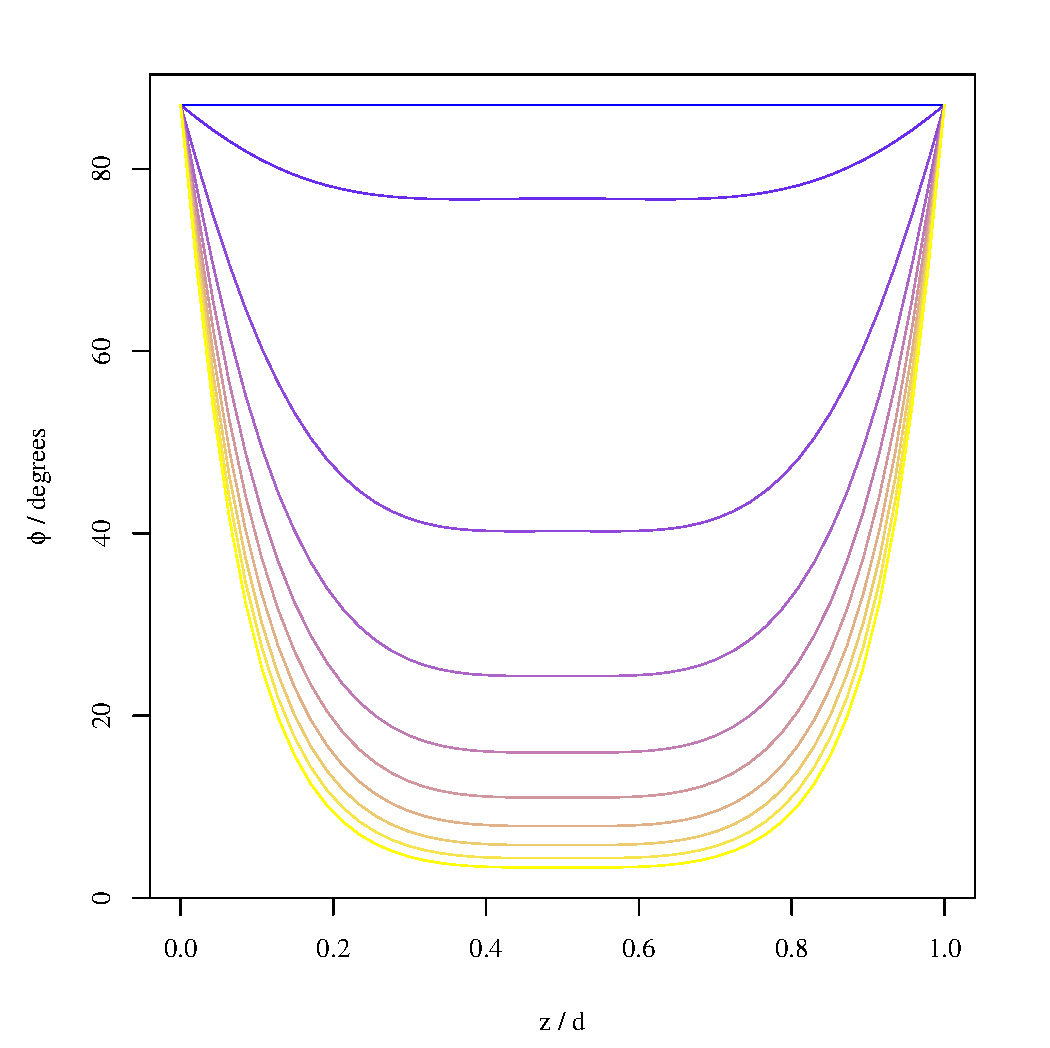
\includegraphics[width=0.49\textwidth]{Figures/45/twist_profile}}
\subfigure[Tilt profile]{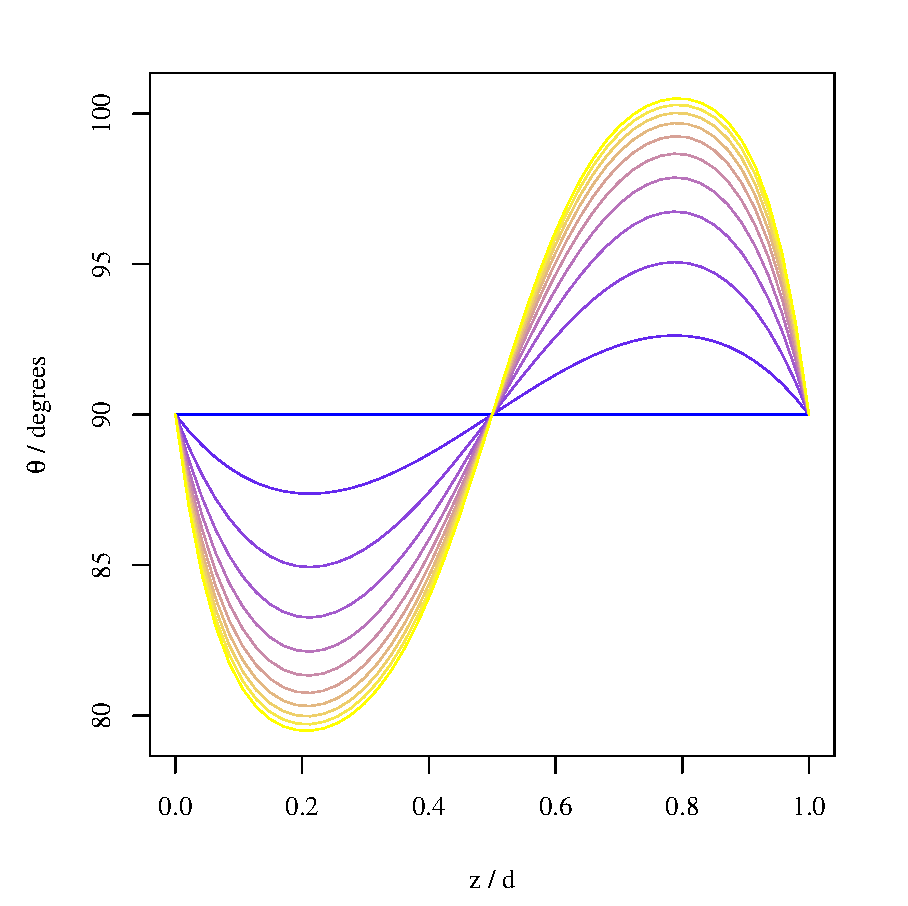
\includegraphics[width=0.49\textwidth]{Figures/45/tilt_profile}}
\subfigure[Velocity profile]{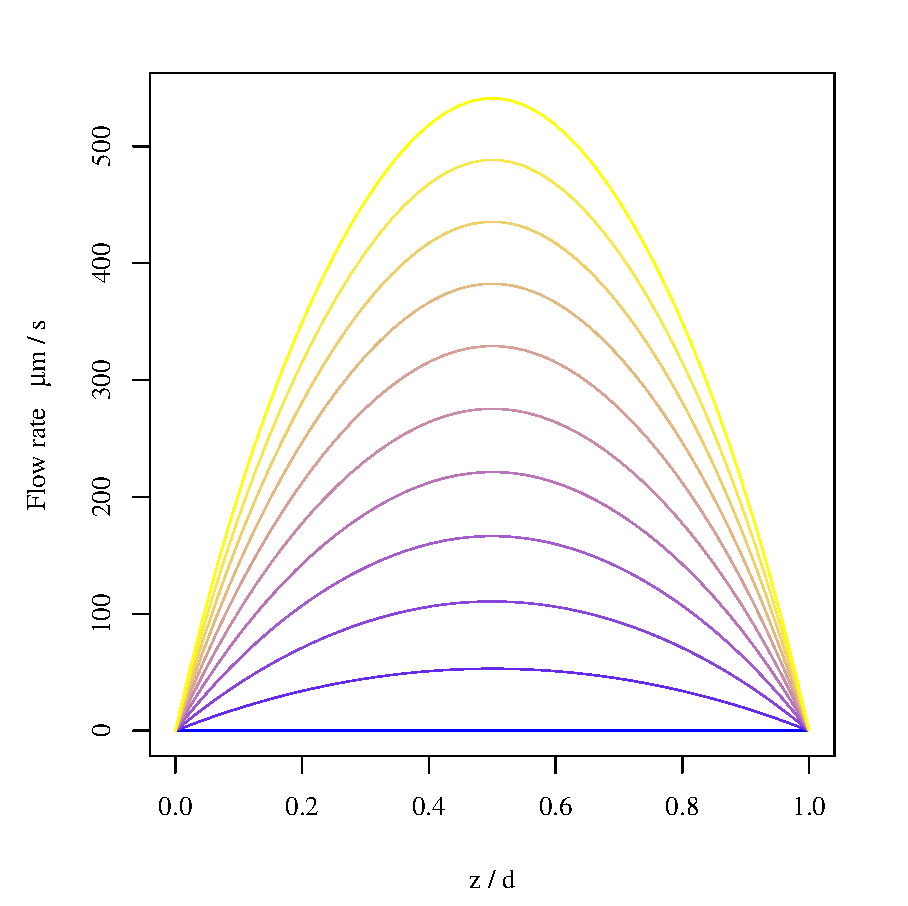
\includegraphics[width=0.49\textwidth]{Figures/45/velocity_profile}}
\end{center}
\caption[Simulated twist, tilt and velocity profiles ($\phi_0=45^{\circ}$)]{\label{fig:twist_tilt_profile} Azimuthal `twist' (a), zenith `tilt' (b) and velocity profiles (c) as a function of cell depth and volumetric flow rate (calculated from the simulated pressure gradient). All three figures show curves at regular intervals from blue (no flow) to yellow (maximum flow), going through orange. (a) Azimuthal rotation is simulated to be symmetric about $z=d/2$ with the whole cell rotating towards $\phi=0^{\circ}$ apart from at the cell boundaries. (b) Tilt distortions are also seen to be symmetric about $z=d/2$ as schematically shown in Figure \ref{fig:c_p} (b), with the director saturating at the Leslie angle in the bottom and top halves of the cell. (c) Simulated, symmetric about $z=d/2$, velocity profiles. For the maximum volumetric flow rate, a fluid velocity of approximately 500 $\mu m/s$ is shown at $z=d/2$.}
\end{figure}

\subsection{Torque balance}
An understanding of the $\phi$ and $\theta$ rotations shown in Figure \ref{fig:twist_tilt_profile} can be gained from analysis of the torque balance equations introduced in Chapter \ref{sec:theory}. In order to do this, one must consider the final term in the $\phi$ torque balance (Equation \ref{eq:phi}), shown below.

\begin{equation}
\frac{1}{2}\alpha_2\sin2\theta\left(\cos\phi\frac{\partial u_y}{\partial z}-\sin\phi\frac{\partial u_x}{\partial z}\right)
\end{equation}

This term is seen to be the only term that drives the director azimuthal rotation as a result of the velocity gradients in the cell, that is to say, this term governs the azimuthal rotation of the director induced by the flow. Firstly, if we consider, as is shown by the director tilt profile Figure \ref{fig:twist_tilt_profile}(b), that under flow the director is always aligned planar $\left(\theta=90^{\circ}\right)$ at $z=0$, $z=d/2$ and $z=d$. Therefore from the final term in equation \ref{eq:phi},

\begin{equation}
\frac{1}{2}\alpha_2\sin2\theta=\frac{1}{2}\alpha_2\sin(180)=0
\end{equation}

we see that the $\phi$ torque balance goes to zero. Therefore, at the cell boundaries and the cell mid-plane, there is no flow-induced torque creating a $\phi$ rotation of the liquid crystal. However, at positions in the cell depth other than the boundaries and cell mid-plane, the value of $|\sin2\theta|$ will have two maxima, one at $z_1$ and one at $z_2$. In this case, $0<z_1<d/2$ and $d/2<z_2<d$. If we now assume that $\theta$ varies evenly as a function of cell depth, the location of these maxima will be close to $z_1=d/4$ and $z_2=3d/4$. That is to say that the maximum distortion in $\theta$ will occur at approximately one quarter and three quarters of the way through the cell. This is demonstrated in Figure \ref{fig:twist_tilt_profile}(b) where the director saturates at the Leslie angle at approximately these depths\footnote{The precise location of the maxima will depend on the various elastic and viscous coefficients}. This is also show in Figure \ref{fig:leslie_angle} where the tilt angle as a function of flow rate is shown for depths of $z=d/4$ (red line) and $z=3d/4$ (blue line).

Therefore we can expect that $\phi$ will vary quickly in $z$ from its strongly anchored boundary condition at $z=0$ to $z=d/4$ and again from its strongly anchored condition at $z=d$ to $z=3d/4$. In both cases, $\phi$ will vary from $\phi_0\left(z=0\right)$ to $\phi_1\left(z_1\right)$ and $\phi_0\left(z=d\right)$ to $\phi_2\left(z_2\right)$ where $\phi_1=\phi_2$. Now, as is shown above, there is no flow induced torque driving the director distortion at $z=d/2$, and therefore only the elastic contribution needs to be considered. As such, we would expect $\phi\left(z=d/2\right)=\phi_1=\phi_2$, that is, the value of $\phi$ at the mid-plane of the cell to equal the maximum distortion of $\phi$ at $z=d/4$ and $z=3d/4$, as is shown in \ref{fig:twist_tilt_profile}(a).

Note that in a cell where the director is confined to be uniformly aligned at exactly $\theta=90^{\circ}$ (the final term of the $\phi$ torque balance goes to zero), there would be no azimuthal rotation of the director at all. This implies, as was suggested by the analysis of the Pieranski-Guyon instability in Section \ref{pg_instability}, that there must be a small component of the director out of the $x-y$ plane in order for there to be any azimuthal rotation of the director.

\begin{figure}
\begin{center}
\includegraphics[width=0.65\textwidth]{Figures/45/leslie_angle}
\end{center}
\caption[Simulated tilt angle of the director saturating at $\theta_l$ at $z=d/4$ and $z=3d/4$]{\label{fig:leslie_angle}A plot showing the simulated tilt angle at $z=d/4$ (red line) and $z=3d/4$ (blue line) approaching saturation at the Leslie angle (dashed lines) as a function of the volumetric flow rate. The black line shows the mathematical mean value of the tilt angle.}
\end{figure}

\begin{figure}
\begin{center}
\subfigure[ 0 $\mu$L/h]{\includegraphics[width=0.18\textwidth]{Figures/45/data00}}
\subfigure[ 0 $\mu$L/h]{\includegraphics[width=0.18\textwidth]{Figures/45/model/00}}\\
\subfigure[ 10 $\mu$L/h]{\includegraphics[width=0.18\textwidth]{Figures/45/data02}}
\subfigure[ 10 $\mu$L/h]{\includegraphics[width=0.18\textwidth]{Figures/45/model/15}}\\
\subfigure[ 20 $\mu$L/h]{\includegraphics[width=0.18\textwidth]{Figures/45/data04}}
\subfigure[ 20 $\mu$L/h]{\includegraphics[width=0.18\textwidth]{Figures/45/model/31}}\\
\subfigure[ 30 $\mu$L/h]{\includegraphics[width=0.18\textwidth]{Figures/45/data06}}
\subfigure[ 30 $\mu$L/h]{\includegraphics[width=0.18\textwidth]{Figures/45/model/47}}\\
\subfigure[ 40 $\mu$L/h]{\includegraphics[width=0.18\textwidth]{Figures/45/data08}}
\subfigure[ 40 $\mu$L/h]{\includegraphics[width=0.18\textwidth]{Figures/45/model/63}}\\
\subfigure[ 50 $\mu$L/h]{\includegraphics[width=0.18\textwidth]{Figures/45/data10}}
\subfigure[ 50 $\mu$L/h]{\includegraphics[width=0.18\textwidth]{Figures/45/model/79}}
\end{center}
\caption[Comparison between experimental and simulated conoscopic figures ($\phi_0=45^{\circ}$)]{\label{fig:45_model_data} A comparison between the experimental and simulated conoscopic figures. Experimental figures are shown in the column on the left and simulated figures are shown in the column on the right. Both are shown for the volumetric flow rate given in the individual figure caption.}
\end{figure}

\subsection{Experimentally varying}
As a small extension to this study, Figure \ref{fig:time_relax} (a) shows further experimental data detailing the angle of conoscopic figure rotation as a function of volumetric flow rate for different flow cells. Here, the flow induced director distortion in cells rub aligned (identically to that described in Section \ref{sec:45_experiment}) at angles of $\phi_0\approx90^{\circ}$ and $\phi_0=0^{\circ}$ are shown. As before, cells were constructed and conoscopic figures were taken at a series of volumetric flow rates set by the syringe drive, allowing determination of the rotation angle and hence the average azimuthal distortion of the director in the cell.

As expected, for the case where the director is initially aligned at $\phi_0\approx90^{\circ}$ (triangles), the average distortion of the director is seen to rotate into the flow direction towards the steady state alignment angle of $\phi=0^{\circ}$\footnote{Note that for this data set $\left(\phi_0\approx89^{\circ}\right)$ there is only a small indication of the Pieranski-Guyon instability as shown in Figure \ref{fig:Pieranski_Guyon_instability}. The lack of instability is likely due to the pretilt as is discussed later in Section \ref{sec:45_vary_tilt}}. For the case where the director is initially aligned at $\phi_0=0^{\circ}$ (circles), there is no observed rotation of the conoscopic figure (due to the director starting in the steady state condition). These results agree well with the theory described by Ericksen and Leslie as well as previous results obtained by Boudreau \textit{et al} \cite{Boudreau1999} for shear driven flow of the liquid crystals 5CB and MBBA.



\section{Terminating flow}
\label{sec:stop_flow}
As was mentioned in Section \ref{sec:analysis}, when the flow is stopped, there is no longer any flow induced torque acting on the director. As such, the competing torques are no longer in balance, with the only component of torque coming from the elastic restoration of the surface aligning layer. At the cell boundary, the director is strongly anchored to be aligned at $\phi=45^{\circ}$, but away from the cell boundaries, at high flow rates, the director is rotated into the flow direction as shown in Figure \ref{fig:twist_tilt_profile}(a). The resulting reaction when the flow is terminated is for the director to rotate back to its initial alignment angle of $\phi_0=45^{\circ}$ under force from the elastic distortion created by the flow alignment. Figure \ref{fig:time_relax} (b) shows a plot of the conoscopic figure rotation angle as a function of time, with $t=0$ being the moment that the flow is terminated\footnote{The data for this plot is not taken from the same cell that the data from Figure \ref{fig:45_data_plot} is taken, but rather a new cell made much later on.}. Inherently, it is difficult to make this measurement due to the conoscopic figure rotating back to it's initial alignment within approximately 15 seconds. Figure capture and storage was not possible on this time scale. In order to take these measurements, a video of the rotation was captured, whereby a cocktail stick was introduced into the field of view at the same time that the flow was terminated. This way, when playing back the footage, $t=0$ could be identified.

\begin{figure}
\begin{center}
\subfigure[]{\includegraphics[width=0.55\textwidth]{Figures/45/0,45,90}}
\subfigure[]{\includegraphics[width=0.55\textwidth]{Figures/45/time_relax}}
\end{center}
\caption[Conoscopic figure rotation for different $\phi_0$ and terminating flow]{\label{fig:time_relax} (a) Data taken from cells fabricated in this study. For cells initially rubbed at $\phi_0\approx89^{\circ}$, $\phi_0=45^{\circ}$ and $\phi_0=0^{\circ}$ (the value of $\psi$ at 0 $\mu$L/h), rotation of the conoscopic figure is observed. For the cell with initial alignment of $\phi_0=0^{\circ}$, no rotation of the conoscopic figure is observed. This is explained by the fact that the director is initially in the steady state condition. (b) Relaxation of the conoscopic figure. Flow is switched off (from a volumetric rate of 100 $\mu$L/h) and the figure's rotation angle $\psi$ is plotted as a function of time. Time = 0 s indicates the moment at which the pump is stopped. It is demonstrated that the figure rotates back to it's initial alignment of $\phi_0\approx45^{\circ}$ within approximately 20 seconds of the pump being switched off. Note that this data is taken from a different cell than the one used to extract the data for Figure \ref{fig:45_data_plot}.}
\end{figure}


Figure \ref{fig:time_relax} shows that within approximately 15 seconds, the director has rotated back to the original alignment state, and we also observe that the conoscopic figure has returned to its initial image. As mentioned in Pieranski's paper of 1974 \cite{Pieranski1974}, the result that the conoscopic figure returns to the initial state when the flow is stopped is essential in describing the process which leads to the observed flow alignment. In this case, it is clear that no permanent deformation of the aligning layer has occurred due to the pressure induced flow in the cell.

\section{Further simulation}
\label{sec:45_vary_tilt}
The one dimensional model used for the simulation of the director distortion in this chapter can also be used to easily simulate pressure driven flow under different director alignment conditions. As a tool, it is extremely powerful and useful in enabling the user to edit all of the parameters and subsequently simulate the corresponding director dynamics under flow. As will be discussed much later in this Thesis (Chapter \ref{cha:pretilt}) the application and control of surface pretilt of the director can be used to have desirable effects on LCD response and dynamic behaviour, along with the methods and techniques that can be used to produce such pretilt angles. 

This section gives a brief introduction to the effect that pretilt can have on the flow alignment of the director. Figure \ref{fig:45_vary_tilt} depicts the same mean azimuthal distortion curve shown for $\phi_0=45^{\circ}$ in Figure \ref{fig:time_relax} (a), along with a series of other curves whereby the director profile is not set to be uniformly aligned at $\theta=90^{\circ}$ through the cell depth, but is rather tilted in at both surfaces, so that a splayed, linearly varying director profile (planar at $z=d/2$) is considered. As stated in the key, the value of the pretilt angle is given here, from the surface, so that a value of $0^{\circ}$ (black line) is planar, and a value of $10^{\circ}$ (red line) has the director tilted away from each surface by $10^{\circ}$, to create a splay of the director as schematically depicted in Figure \ref{fig:s,t,b} (a).

 
\begin{figure}
\begin{center}
\subfigure[]{\includegraphics[width=0.49\textwidth]{Figures/45/vary_tilt}}
\subfigure[]{\includegraphics[width=0.49\textwidth]{Figures/45/pieranski_pretilt}}
\end{center}
\caption[Simulations of applied pretilt on the Pieranski-Guyon instability]{\label{fig:45_vary_tilt} (a) A plot of the computed mean azimuthal rotation of the director as a function of volumetric flow rate and pretilt angle for an azimuthal alignment of $\phi_0=45^{\circ}$. The legend shows the amount of pretilt, \textit{in this case measured from the surface}, in the splayed geometry (the director is always planar at $z=d/2$). As the amount of pretilt is increased, the transient portion of the curve steepens, and much of the director rotation is achieved at lower flow rates. (b) The same result is shown for the Pieranski-Guyon instability. Here, a pretilt angle of 1$^{\circ}$ removes all trace of the threshold velocity. This result comes from the fact that the initial azimuthal torque on the director is larger for a starting condition of higher pretilt.}
\end{figure}

It is clear from Figure \ref{fig:45_vary_tilt} that as the degree of pretilt is increased, the rate of azimuthal rotation is also increased, with a more sensitive response at lower flow rates. For the case of 20$^{\circ}$ of pretilt of the director (grey line) a larger azimuthal response is observed (shown best in the magnified area of the graph). Here, it is clear that for the same volumetric flow rate, the director has rotated far more away from the initial alignment angle. It is also shown that at larger flow rates, the average azimuthal director rotation is larger in the case of a larger pretilt angle.

This simulated response makes good quantitative sense if the argument behind flow alignment suggested by Pieranski and Guyon \cite{Pieranski1974} (Section \ref{pg_instability}) is considered. As the initial director field is further tilted out of the $x-y$ plane (a higher pretilt value), there is already a larger component of the individual molecule tilted into the velocity gradient created by the pressure driven flow. Therefore, the azimuthal torque on the molecules is much larger for any given flow rate when larger pretilt angles are considered. This is demonstrated by the curves in Figure \ref{fig:vary_tilt} showing more rotation as the pretilt angle is increased. Figure \ref{fig:vary_tilt} (b) shows that just a small amount of pretilt will remove the threshold flow rate needed in order to create the flow instability. This is demonstrated by there being no sharp turning point in Figure \ref{fig:45_vary_tilt} (b) for the curves that are simulated using a small amount of pretilt.

The effect of pretilt angle on flow will be discussed at length in the next chapter, whereby different arrangements of pretilt can be shown to have a striking effect on the overall director response to flow.

\section{Conclusions}
This chapter has looked at the pressure driven flow alignment of the liquid crystal 5CB originally aligned planar homogeneously at an azimuthal angle of $45^{\circ}$ to the direction of flow. Conoscopy has been used to measure the average azimuthal alignment of the sample as a function of the volumetric flow rate set at the syringe drive and has been compared to simulation from the one dimensional dynamic model based on the theory of Ericksen and Leslie. 

Conoscopic figure rotation suggests that under flow, the director has rotated to achieve an angle close to the direction of the flow, whilst conoscopic figure translation suggests that the director has tilted to form a splayed director profile saturating at the Leslie angle of opposite signs in both halves of the cell. This result is in good agreement with the simulation.

Flow alignment for samples aligned at both $\phi_0\approx90^{\circ}$ and $\phi_0\approx0^{\circ}$ have also been observed to flow align, with the sample aligned at $\phi_0\approx90^{\circ}$ to the flow direction rotating to come in line with the flow, and the sample aligned at $\phi_0\approx0^{\circ}$ showing no rotation (due to the fact that it is already aligned parallel to the direction of flow).

The good agreement between simulation and data suggests that the quoted viscosity coefficients (Table \ref{tab:visc}) for 5CB are reliable.
